\section{Evaluation}
We cannot rely on traditional approaches such as manual
labeling to evaluate large-scale performance.  We therefore sought to
minimize failure rate, quantify the repeatability of cortical
thickness measures, test accuracy in BrainAGE \citep{franke2010}, and
determine whether the DiReCT pipeline reveals biologically plausible relationships
between the cortex, age, and gender.  Collectively, these surrogate
measurements allow us to establish data-derived performance standards.

\subsection{Computation Time and Failure Rate}
All images underwent the pipeline processing illustrated in Figure 
\ref{fig:pipeline} using the computational cluster at the University 
of Virginia.%
\footnote{
http://www.uvacse.virginia.edu/itc-clusters/
}  
Processing times varied approximately between 10--20 hours per subject
for the entire cortical thickness estimation procedure.  The propagation of the
NIREP labels to each subject using label fusion as described earlier
was performed in parallel and took anywhere between 40 and 80 hours per 
subject for 16 serial image registrations and application of the joint label fusion algorithm \citep{wang2013}.%
\footnote{
All processing on the UVA cluster was set to be single-threaded with a maximum requested memory footprint of 8 GB.  See script for exact cluster commands.
}  
Average thickness values were tabulated per subject for each of the
32 NIREP labels.  Cerebral volumes for each subject derived from the brain 
extraction step were also calculated.  All these data were written to separate csv
files corresponding to data set for subsequent 
analysis (also included with the scripts).  Visual sample results from each data set are provided in 
Figure \ref{fig:sampleResults}.

No obvious brain extraction failures (e.g. frontal lobe mask leaking into 
the eyes) were detected during the course of this study.  
Quality assessment was done manually by multiple rounds of visual inspection using 
ITK-SNAP \cite{yushkevich2006}.  Similarly, we detected no obvious segmentation errors.  Brain constellation maps (detailed in a later section)
provided a unified view of all thickness results for the entire cohort for
a quick quality check.

\begin{figure*}[htb]
  \begin{center}
  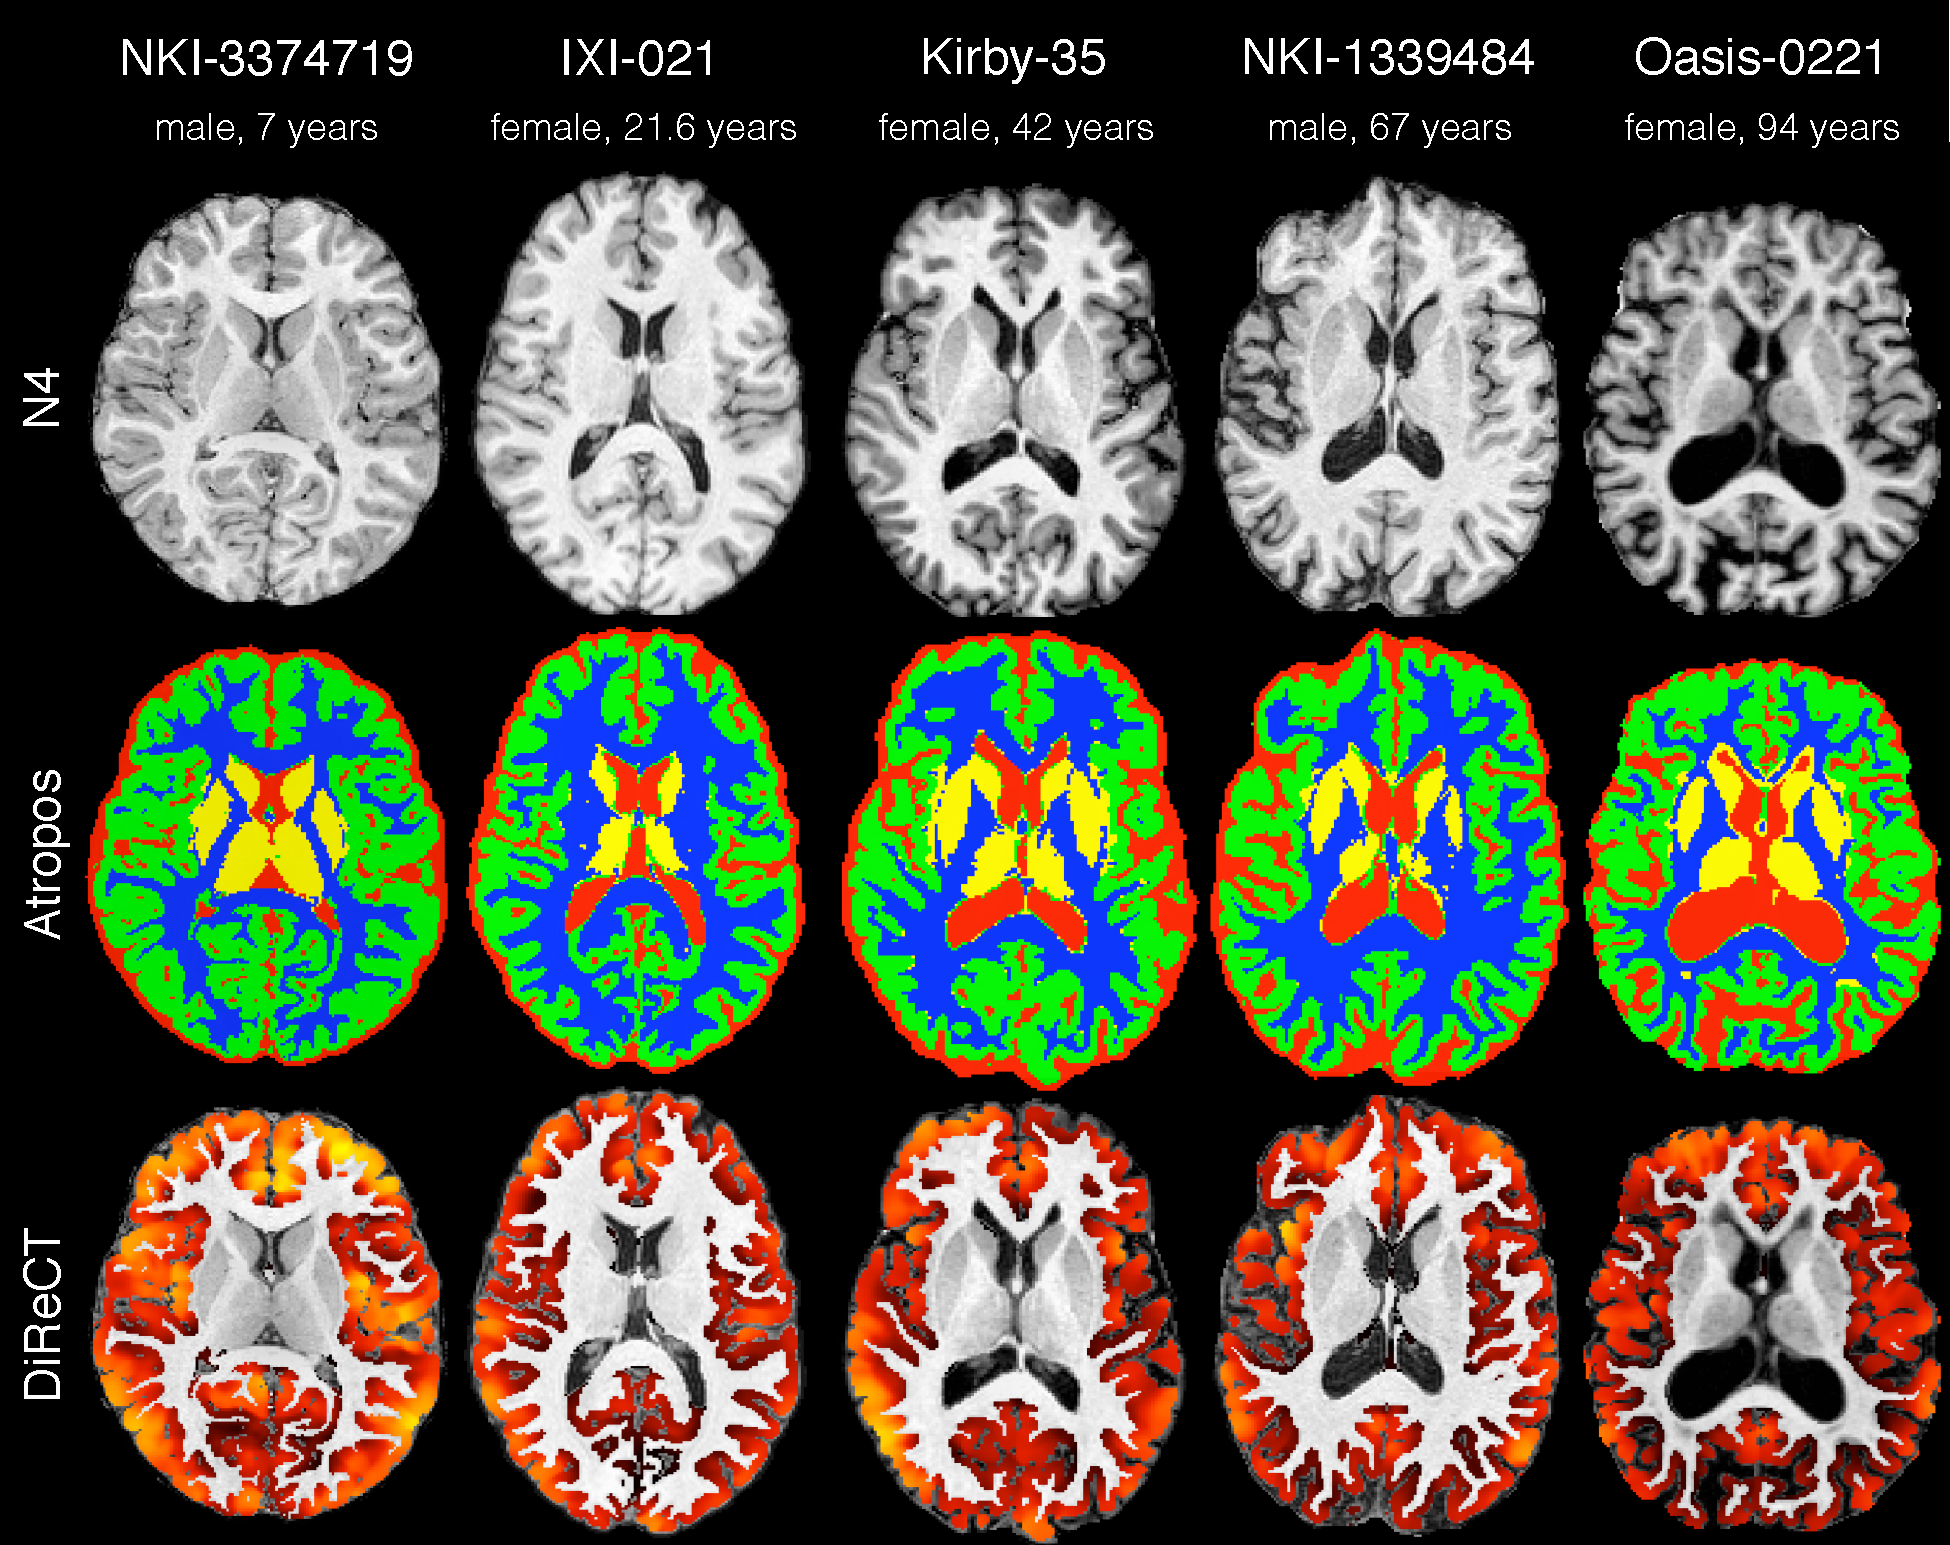
\includegraphics[width=120mm]{sampleVisualResults.pdf}
  \caption{Sample results from each of the four data sets showing the N4 bias
  corrected images, 4-tissue segmentation, and cortical thickness
  maps. }
  \label{fig:sampleResults}
  \end{center}
\end{figure*}
  
  
\subsection{Reproducibility}%

\begin{table*}
\centering
\begin{tabular*}{\textwidth}{@{\extracolsep{\fill}} l c c c c}
\toprule
\multicolumn{1}{c}{} & \multicolumn{2}{c}{Absolute Difference (mm)} & \multicolumn{2}{c}{Percent Variability Error} \\
\multicolumn{1}{c}{Region} & \multicolumn{1}{c}{Left} & \multicolumn{1}{c}{Right} & \multicolumn{1}{c}{Left} & \multicolumn{1}{c}{Right} \\
%\midrule
%occipital & $0.16 \pm 0.21$ & $0.17 \pm 0.22$ & $5.36 \pm 6.92$ & $5.79 \pm 7.17$\\
%cingulate & $0.12 \pm 0.13$ & $0.12 \pm 0.14$ & $3.7 \pm 4.49$ & $3.62 \pm 4.6$\\
%insula & $0.18 \pm 0.17$ & $0.17 \pm 0.17$ & $4.52 \pm 4.27$ & $4.43 \pm 4.36$\\
%temporal pole & $0.23 \pm 0.23$ & $0.21 \pm 0.2$ & $4.93 \pm 5.48$ & $4.81 \pm 5.01$\\
%superior temporal & $0.13 \pm 0.15$ & $0.1 \pm 0.13$ & $4.74 \pm 5.34$ & $3.58 \pm 4.92$\\
%infero temporal & $0.26 \pm 0.32$ & $0.24 \pm 0.31$ & $6.86 \pm 8.8$ & $6.58 \pm 9.21$\\
%parahippocampal & $0.2 \pm 0.19$ & $0.18 \pm 0.15$ & $5.13 \pm 5.29$ & $4.61 \pm 3.76$\\
%frontal pole & $0.23 \pm 0.24$ & $0.24 \pm 0.25$ & $7.1 \pm 8.07$ & $7.4 \pm 8.32$\\
%superior frontal & $0.11 \pm 0.12$ & $0.12 \pm 0.12$ & $3.86 \pm 4.48$ & $3.85 \pm 4.31$\\
%middle frontal & $0.17 \pm 0.2$ & $0.16 \pm 0.21$ & $6.58 \pm 7.8$ & $5.87 \pm 7.96$\\
%inferior & $0.12 \pm 0.15$ & $0.12 \pm 0.16$ & $4.53 \pm 5.53$ & $4.26 \pm 5.49$\\
%orbital frontal & $0.16 \pm 0.2$ & $0.19 \pm 0.18$ & $4.77 \pm 6.12$ & $5.39 \pm 5.36$\\
%precentral & $0.11 \pm 0.11$ & $0.11 \pm 0.13$ & $4.46 \pm 4.5$ & $4.15 \pm 4.81$\\
%superior parietal & $0.09 \pm 0.1$ & $0.09 \pm 0.09$ & $3.71 \pm 4.14$ & $3.67 \pm 3.78$\\
%inferior parietal & $0.14 \pm 0.17$ & $0.13 \pm 0.18$ & $4.96 \pm 6.06$ & $4.96 \pm 6.74$\\
%postcentral & $0.13 \pm 0.16$ & $0.14 \pm 0.14$ & $5.51 \pm 6.32$ & $6.02 \pm 6.01$\\
\midrule
occipital & $0.14 \pm 0.14$ & $0.16 \pm 0.19$ & $3.57 \pm 3.8$ & $4.13 \pm 4.81$\\
cingulate & $0.07 \pm 0.08$ & $0.09 \pm 0.09$ & $2.18 \pm 2.48$ & $2.63 \pm 2.9$\\
insula & $0.08 \pm 0.05$ & $0.09 \pm 0.1$ & $2.37 \pm 1.6$ & $2.54 \pm 3.01$\\
temporal pole & $0.21 \pm 0.14$ & $0.19 \pm 0.15$ & $3.98 \pm 3.04$ & $3.89 \pm 3.56$\\
superior temporal & $0.08 \pm 0.07$ & $0.07 \pm 0.06$ & $2.83 \pm 2.31$ & $2.54 \pm 2.36$\\
infero temporal & $0.2 \pm 0.25$ & $0.19 \pm 0.24$ & $4.34 \pm 5.82$ & $4.49 \pm 6.38$\\
parahippocampal & $0.19 \pm 0.21$ & $0.17 \pm 0.19$ & $4.82 \pm 5.51$ & $4.29 \pm 4.85$\\
frontal pole & $0.17 \pm 0.17$ & $0.17 \pm 0.14$ & $4.97 \pm 4.97$ & $4.42 \pm 3.97$\\
superior frontal & $0.07 \pm 0.06$ & $0.08 \pm 0.06$ & $2.14 \pm 1.91$ & $2.45 \pm 2.05$\\
middle frontal & $0.12 \pm 0.12$ & $0.09 \pm 0.07$ & $3.7 \pm 3.71$ & $2.96 \pm 2.51$\\
inferior & $0.09 \pm 0.09$ & $0.09 \pm 0.08$ & $2.92 \pm 3.15$ & $3.19 \pm 2.68$\\
orbital frontal & $0.11 \pm 0.12$ & $0.13 \pm 0.12$ & $3.19 \pm 3.79$ & $3.66 \pm 3.69$\\
precentral & $0.07 \pm 0.07$ & $0.06 \pm 0.05$ & $2.52 \pm 2.51$ & $2.37 \pm 1.91$\\
superior parietal & $0.07 \pm 0.06$ & $0.07 \pm 0.05$ & $2.45 \pm 2.14$ & $2.62 \pm 1.67$\\
inferior parietal & $0.1 \pm 0.09$ & $0.09 \pm 0.08$ & $3.11 \pm 2.67$ & $2.82 \pm 2.73$\\
postcentral & $0.09 \pm 0.09$ & $0.08 \pm 0.05$ & $3.56 \pm 3.33$ & $3.26 \pm 2.25$\\
\bottomrule
\end{tabular*}
\caption{Mean absolute difference and percent variability error ($\pm$ standard deviation) of repeated 
cortical measurements for both the Oasis and Kirby repeat scans.
These differences were not statistically significant (two-tailed $t$-test
with false discovery rate (FDR) multiple comparisons correction).
}
\label{table:error}
\end{table*}

Repeat scans of 40 subjects (20 Kirby subjects and 20 Oasis subjects) were 
used to determine the reproducibility of regional cortical thickness 
measurements.%
\footnote{
The R script used for this section is {\tt reproducibility.R}.  Data are
located in the csv files {\tt labelresultsK\_pairwise.csv} (Kirby) and 
{\tt labelresultsO\_pairwise.csv} (Oasis).
}
 Similar to the assessment given in \cite{jovicich2013}, we
show regional reproducible thickness measurements, $T$, in terms of the
variability error:
\begin{align}
\varepsilon = \frac{|T_{scan} + T_{rescan}|}{0.5 \times (T_{scan} + T_{rescan})}.
\end{align}
Error values (including absolute mean differences) for the 32 NIREP regions for both the Oasis and Kirby reproducibility data sets
are given in Table \ref{table:error}.  We also calculated the intraclass 
correlation coefficient 
(``ICC(2,1)'' in the notation of \cite{shrout1979}) to assess scan/rescan
reliability which showed reliable agreement ($ICC=0.98$).  Additional regression
testing exploring the effects of site, age, and gender demonstrated no statistically significant effect on regional mean thickness difference.

\subsection{BrainAGE Evaluation}


\begin{table}
\centering
\begin{tabular*}{0.45\textwidth}{@{\extracolsep{\fill}} l c c}
\toprule
\multicolumn{1}{c}{Analysis} & \multicolumn{1}{c}{$r$} & \multicolumn{1}{c}{mean error (years)} \\
\midrule
Gray matter probability & 0.92 & 6.4 \\  
Cortical thickness & 0.90 & 7.25 \\
\bottomrule
\end{tabular*}
\caption{Correlation and mean error values for both the gray matter probability and cortical thickness
{\it BrainAGE} evaluation.}
\label{table:brainAge}
\end{table}

\begin{figure*}[htb]
  \centering
  \begin{tabular}{cc}
  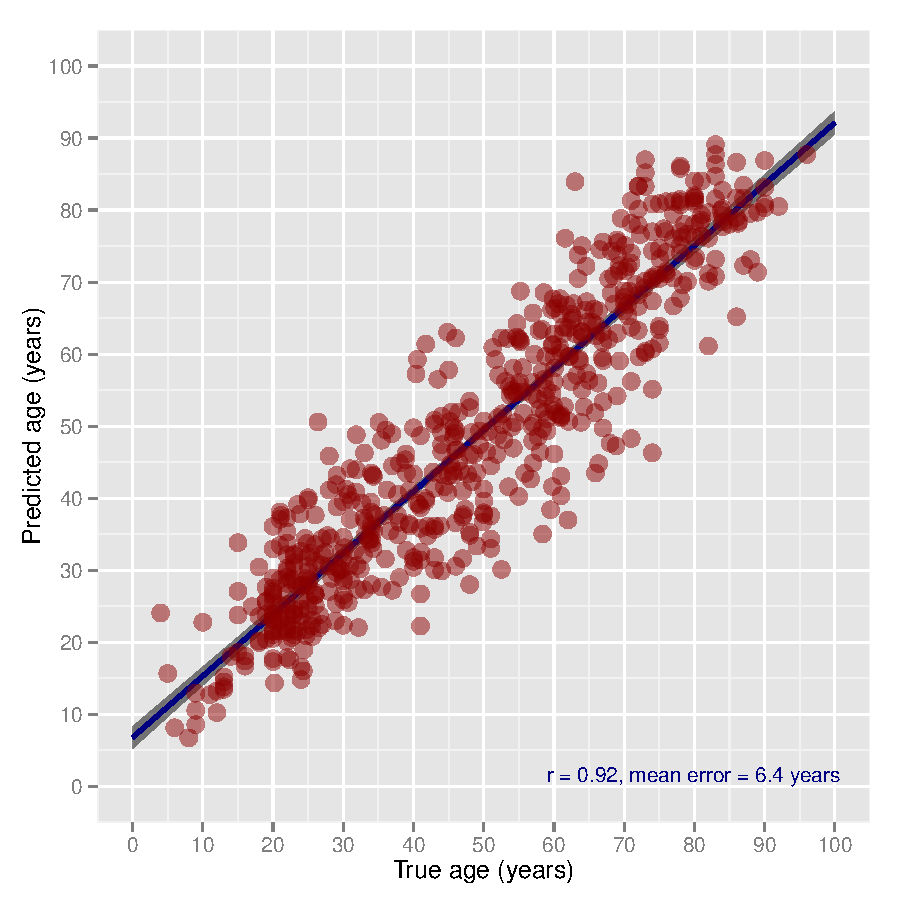
\includegraphics[width=65mm]{brainAgeBrainSegmentationPosteriors2New.pdf} &
  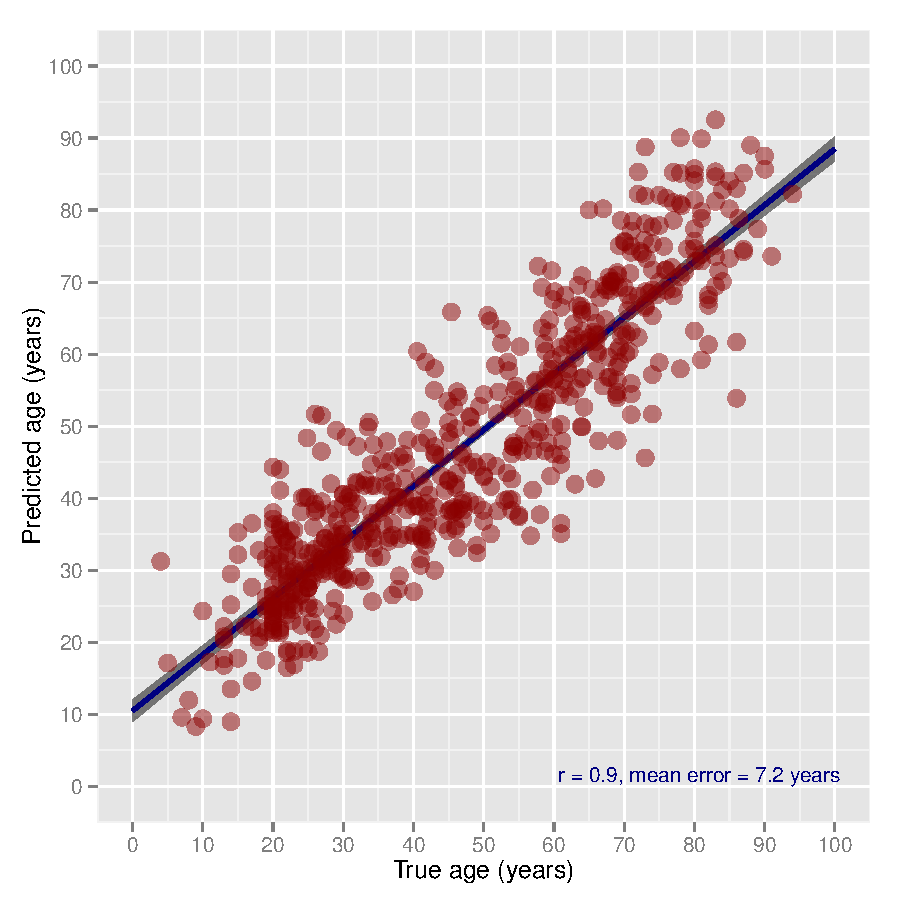
\includegraphics[width=65mm]{brainAgeCorticalThicknessNew.pdf} \\
  (a) & (b) 
  \end{tabular}
  \caption{Results of RVM-based age prediction using (a) gray matter probability
  maps as in \cite{franke2010} and (b) cortical thickness maps both of which
  are derived from the previously described workflow.}
  \label{fig:brainAge}
\end{figure*}

In \cite{franke2010}, an estimation framework is presented for predicting 
apparent age from gray matter segmentation probability maps (denoted by the authors as {\it BrainAGE}).  
Given a normal age population spanning the age range of interest, the authors showed
how kernel regression methods can be used to reliably estimate age.  The basic processing pipeline includes gray matter segmentation
from a subject's T1, followed by affine registration to a common reference space (e.g.
the MNI template), smoothing (8 mm FWHM), and downsampling (8 mm 
isotropic resolution).  A principal components (PCA) model is constructed 
from the resulting aligned training image set.  The images of both the training set and 
testing set are decomposed into the bases of the PCA model which form the feature
set for relevance vector machine (RVM)-based learning and prediction, respectively. 

We applied the BrainAGE framework to the gray matter probability maps derived
from our pipeline.  We also applied the same strategy to predicting age from 
our cortical thickness images.%
\footnote{
The R script used for this section is {\tt brainAgeAnalysis.R}.  Data are
located in the following csv files: 
\begin{itemize}
\item {\tt trainingCorticalThicknessProjections.csv}, 
\item {\tt testingCorticalThicknessProjections.csv},
\item {\tt trainingBrainSegmentationPosteriors2Projections.csv}, and
\item {\tt testingBrainSegmentationPosteriors2Projections.csv}.
\end{itemize}
}  
We randomly separated the images of each of the 
four cohorts into approximately two equal subgroups (testing and training).
Construction of the PCA model and decomposition of all images into the corresponding 
bases were performed on the training group using tools developed from the Insight Toolkit.%
\footnote{
http://www.itk.org/Doxygen/html/classitk\_1\_1ImagePCADecompositionCalculator.html  
}
We used the R package {\it kernlab}%
\footnote{
http://rss.acs.unt.edu/Rdoc/library/kernlab/html/rvm.html
} 
package to train the RVM model and perform prediction.  Results for both
analyses  are shown in Figure \ref{fig:brainAge} (cf Figure 3 in \cite{franke2010}).
The resulting predictions for both image sets are quite similar as demonstrated 
visually in Figure 3.  The correlation coefficients and mean errors in Table 
\ref{table:brainAge} between the
two approaches are also evidence of mutual corroboration.

\subsection{Gender and Age Relationships with DiReCT Cortical Thickness}

\begin{figure}[htb]
  \centering
  \begin{tabular}{c}
  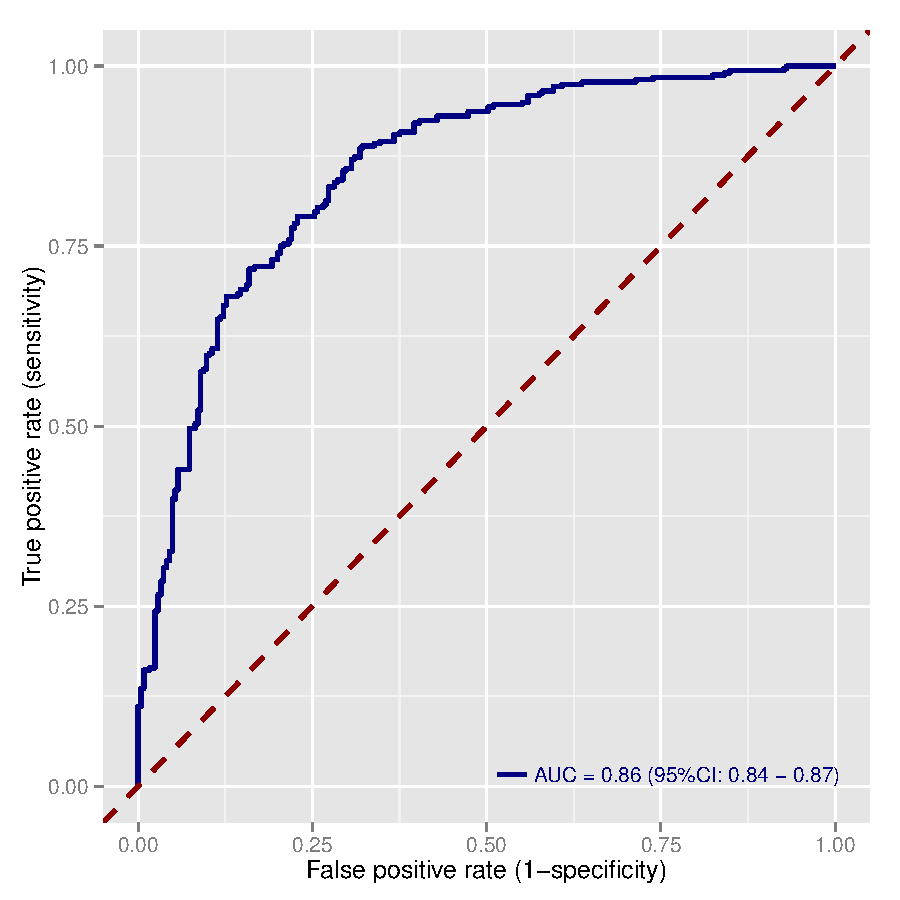
\includegraphics[width=65mm]{sexPlot.pdf} \\
  (a) \\
  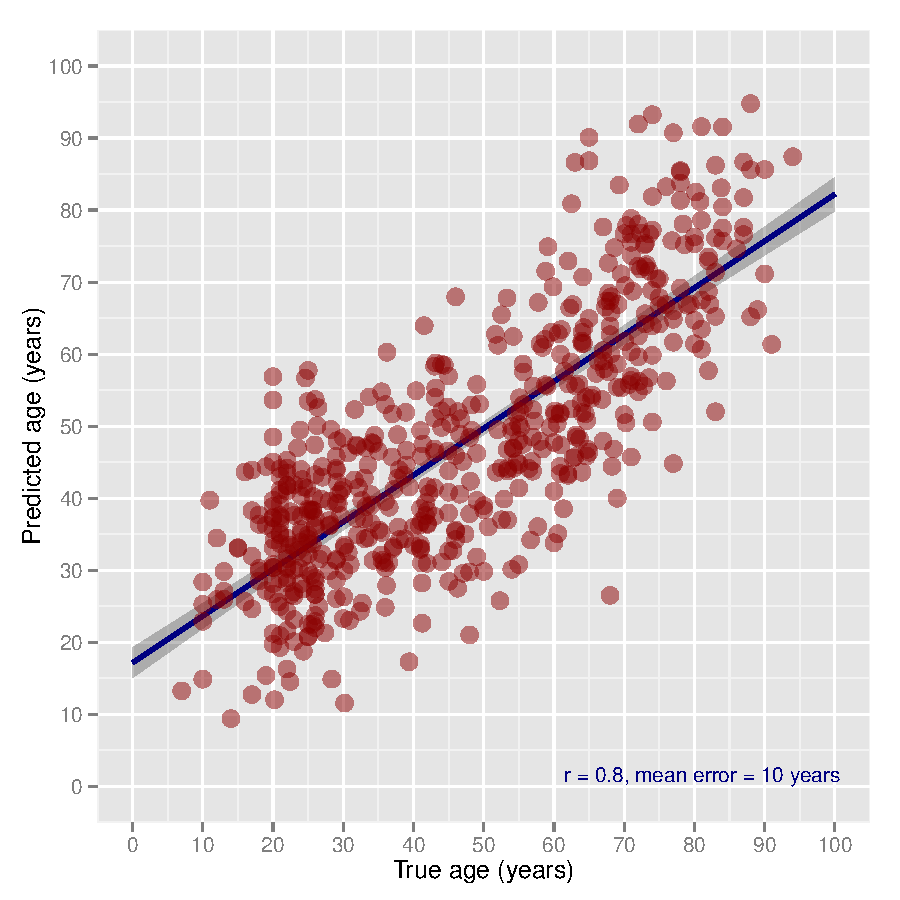
\includegraphics[width=65mm]{ageRegressionPredict.pdf} \\
  (b) 
  \end{tabular}
  \caption{(a) ROC curve based on a gender prediction model using total brain volume and regional thickness values (coupled with cross terms with age---cf Eqn. \ref{eq:roc}).  
  (b) Correlation plot for age prediction using regional thickness.
  }
  \label{fig:sexROC}
\end{figure}

As discussed in the introduction, previous studies have demonstrated 
thickness variation with gender and age which is supported with
the results of our study.  Subdividing the cohort into training and
testing subsets, we generate regression models from the training data
for both gender and age and predict such biological relationships with 
the testing data. Stepwise model selection using Akaike Information Criterion
(AIC) provides an optimal model with minimal parameters.  This provides 
insight into regional thickness importance as well
as the influence of confounds such as site.%
\footnote{
The R scripts for this analysis are {\tt genderThicknessRegression.R} and
{\tt ageThicknessRegression.R}.  Data are located in the following csv files: 
{\tt labelresultsI.csv} (IXI), 
{\tt labelresultsK.csv} (Kirby),
{\tt labelresultsN.csv} (NKI), and
{\tt labelresultsO.csv} (Oasis).
}

We first tested the ability of regional thickness and cerebral volume to determine
gender.
In the notation of \cite{wilkinson1973}, the initial binomial 
generalized linear model is
\begin{align}
  GENDER \sim AGE &+ VOLUME + \sum_{i=1}^{32} T(REGION_{i}) \\ \nonumber
              &+\sum_{i=1}^{32} T(REGION_{i}):AGE
\end{align}
where $T(REGION_{i})$ is the average thickness value in $REGION_{i}$.
The stepwise AIC model selection resulted in the pruned model
\begin{align}
  \label{eq:roc}
  GENDER \sim VOLUME &+ \sum_{i \in \alpha} T(REGION_i) + \\ \nonumber 
                    & \sum_{j \in \beta} T(REGION_j):AGE
\end{align}
where the sets $\alpha = \{1,2,4,7,8,10,12,14,15,19,22,24,27,29,32\}$ and $\beta = \{7,24,27,29\}$ (see Table \ref{table:nirep_labels}).  We then characterized the performance using a ROC curve (see Figure \ref{fig:sexROC}(a)) with AUC = 0.86 and 95\% confidence interval = (0.84, 0.87). 
   
Similarly, a testing/training data partitioning was used to generate a linear model 
and test age prediction by regressing on regional thickness,
cerebral volume, gender, and site resulting in the formula
\begin{align}
  AGE \sim VOLUME + SITE + GENDER + \sum_{i=1}^{32} T(REGION_{i})
\end{align}
with stepwise AIC selection producing the following model
\begin{align}
  AGE \sim SITE + \sum_{i\in\gamma} T(REGION_{i})
\end{align}
where the set $\gamma = \{2,3,7,9,12,13,15,16, 21,23,25,26,27,28,31\}$.  The predicted age vs. true age plot is given
in Figure \ref{fig:sexROC}(b) with Pearson correlation coefficient = 0.77 with a mean
age error of 10 years.


\subsection{Gender Structural Connectivity Across Age Using Cortical Thickness}

%\textcolor{red}{ Nick - should show a rendering of these networks -
%  how about we residualize thickness wrt age and then look at the
%  difference between male and female transitivity?  we can permute to
%  get significance .... } 
%\begin{figure*}
%  \centering
%  \begin{tabular}{c}
%  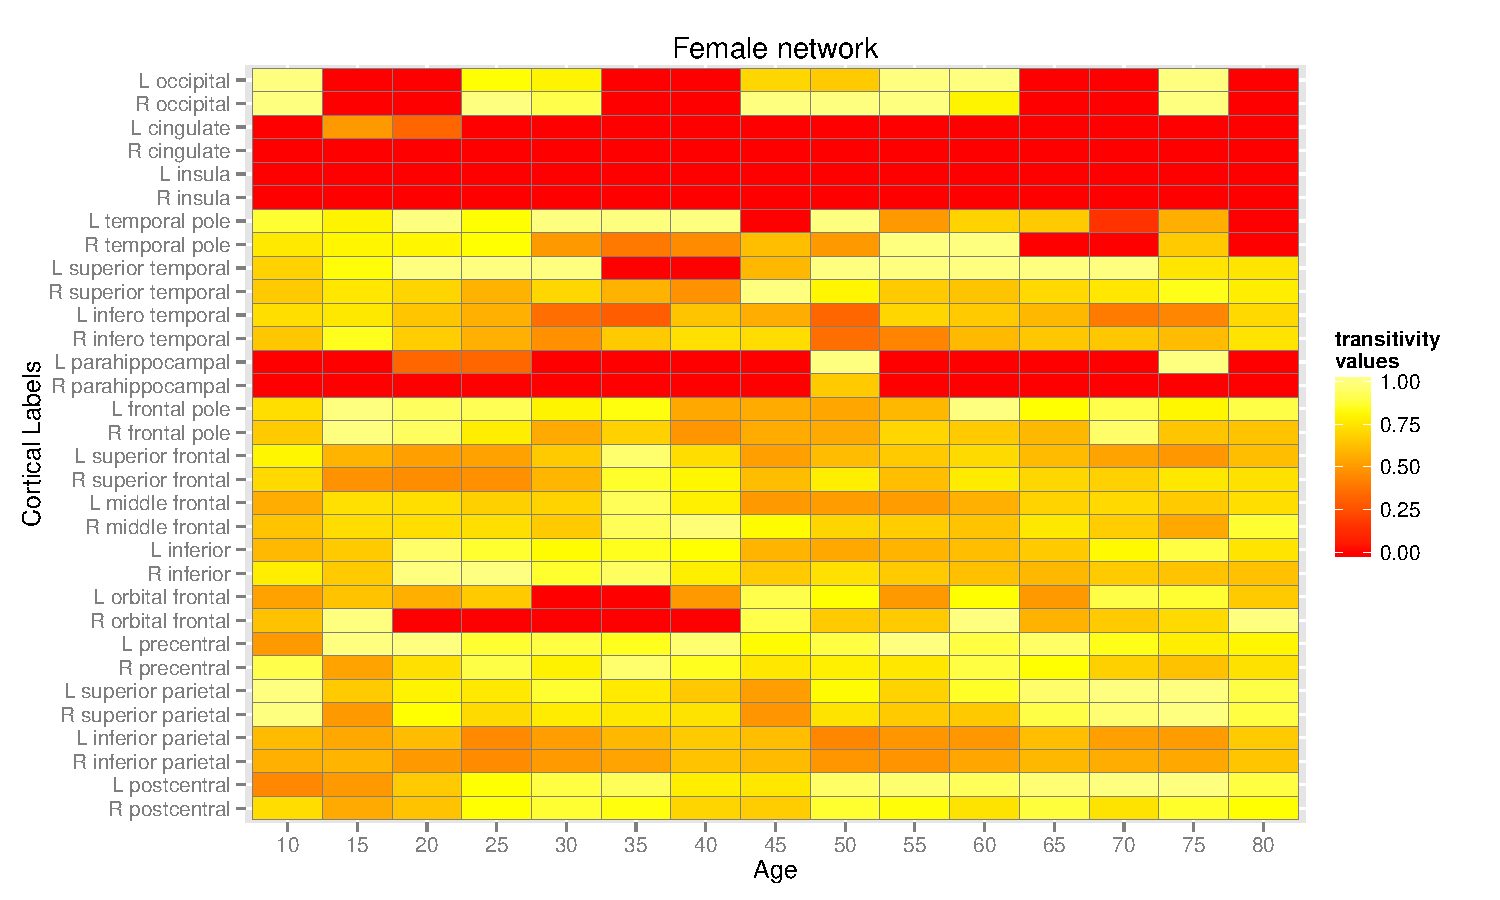
\includegraphics[width=140mm]{femaleNetwork.pdf} \\
%  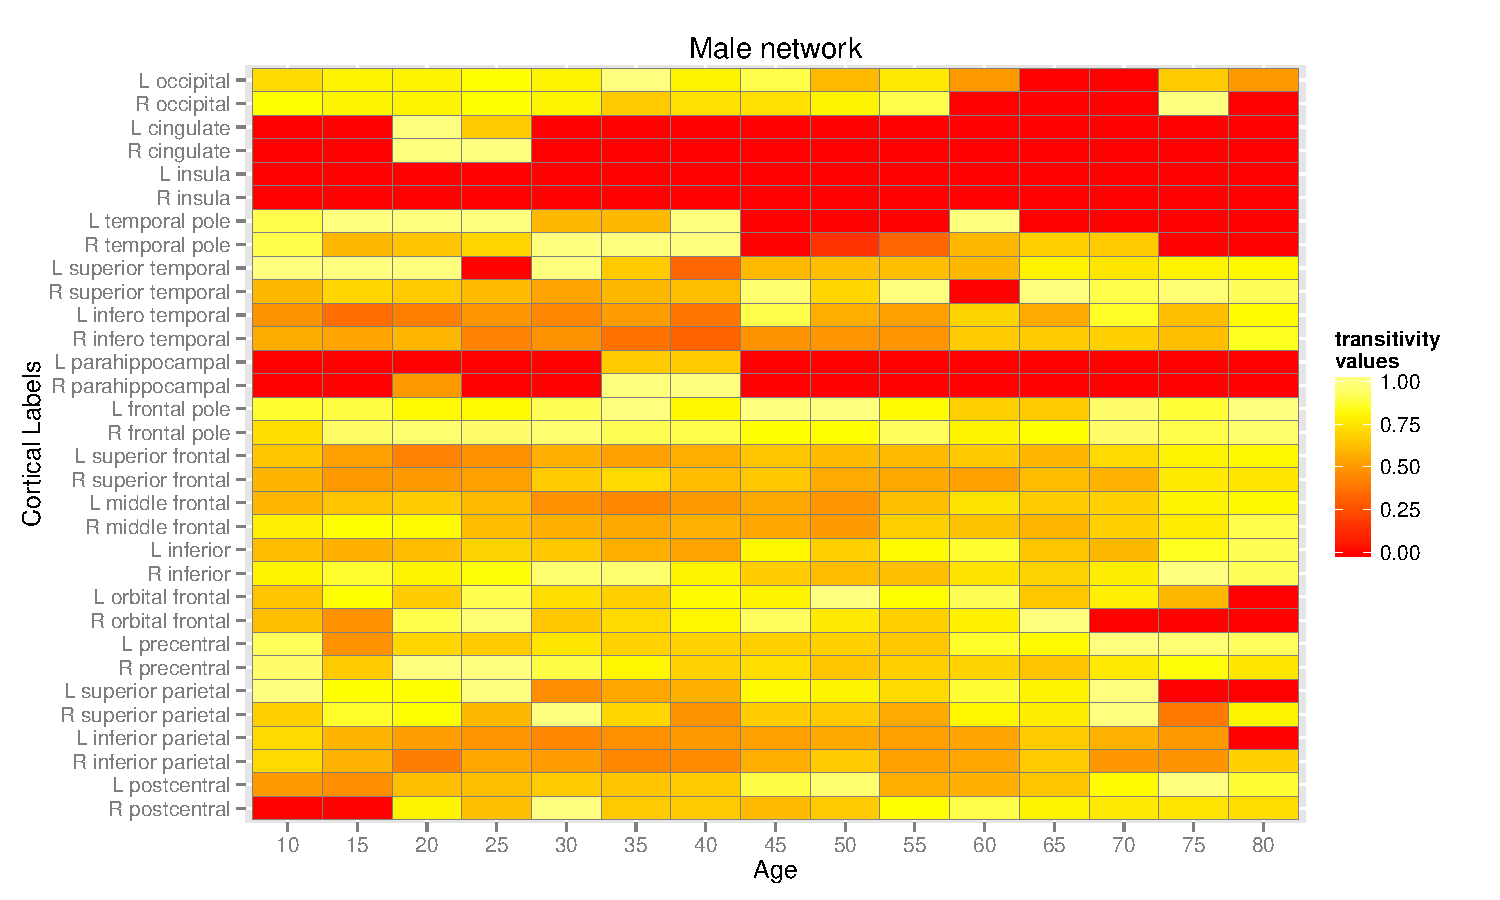
\includegraphics[width=140mm]{maleNetwork.pdf}
%  \end{tabular}
%  \caption{Transitivity (clustering coefficient) values across age for both the female (top)
%  and male (bottom) networks.  
%  }
%  \label{fig:network}
%\end{figure*}

As mentioned in the Introduction, cortical thickness has
been used to determine structural connectivity relationships in the brain 
where strong correlations in regional cortical 
thickness values across subjects provide evidence for anatomical
connectivity \citep{he2007,chen2008,he2008}.  Specifically, networks of neuronal
regions are thought to have small-world network properties \citep{sporns2004} 
in which clustered subnetworks are sparsely connected to other such clusters.
Measures such as the
clustering coefficient (or local transitivity) and mean shortest path length
\citep{watts1998}, are used to characterize networks in terms of their 
small-worldness.
%Although the principal purpose of this work is to showcase the 
%publicly available ANTs cortical thickness pipeline and its performance
%on open data
%(and not necessarily explore the deeper neuroscience implications of 
%the results), 
We use the compiled cortical thickness data to briefly sketch
the longitudinal variation in gender-based small-world networks of the
brain.%
\footnote{
The R scripts for this analysis are {\tt genderStructuralConnectivity.R}.  Data are located in the following csv files: 
{\tt labelresultsI.csv} (IXI), 
{\tt labelresultsK.csv} (Kirby),
{\tt labelresultsN.csv} (NKI), and
{\tt labelresultsO.csv} (Oasis).
}

At each age between 10 and 90 years (in increments of 5), the weighted correlation
matrix for each gender is calculated from the thickness residuals 
(modeling the imaging acquisition site and total brain volume as covariates).  An undirected graph ($V \in$ \{NIREP regions\}, $E \in$ \{all NIREP pairings\})
is constructed from the correlation matrix where the graph density is specified at 25\%, i.e. only the nodal adjacencies corresponding to the top 25\% correlation values are used to create edges.    The local transitivity for a given vertex, $v_i$, with $k_i$ neighbors of the resulting graph is calculated from
\begin{align}
  transitivity(v_i) = \frac{|\{e_{jk}: v_j, v_k \in V, e_{jk} \in E \}|}{k_i (k_i-1)/2}.
\end{align}
Informally, this quantifies the proportion of edges between the neighbors of $v_i$ to the total number of possible edges in the neighborhood to quantify the proximity of the neighborhood to a complete graph.  

We determine the longitudinal transitivity gender differences and determine their
statistical significance using permutation testing ($n = 1000$ permutations).  These statistically significant regional results are given in Table \ref{table:genderDifference}.  
We also visualize these connectivity networks for both female and male within the brain
space and as phylogenetic radial trees in Figures \ref{fig:femaleVisualNetworks} and \ref{fig:maleVisualNetworks}, respectively.

\begin{figure*}[htb]
  \centering
  \begin{tabular}{ccc}
  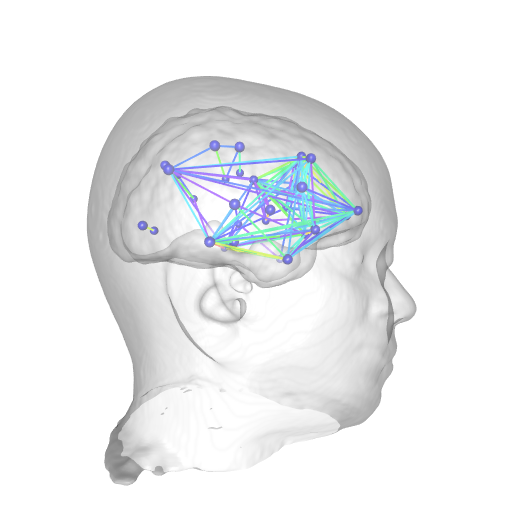
\includegraphics[width=55mm]{temp_female_network_R_20.png} &
  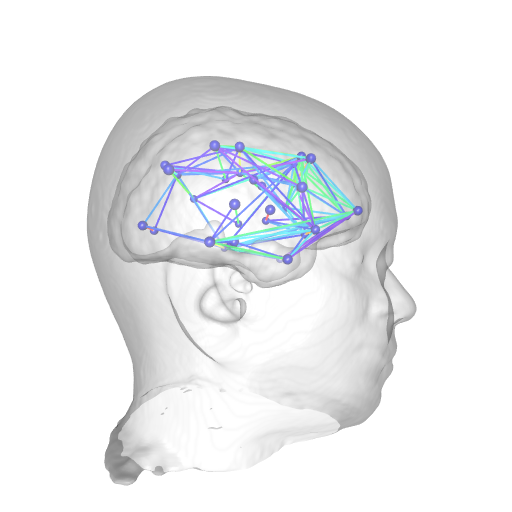
\includegraphics[width=55mm]{temp_female_network_R_40.png} &
  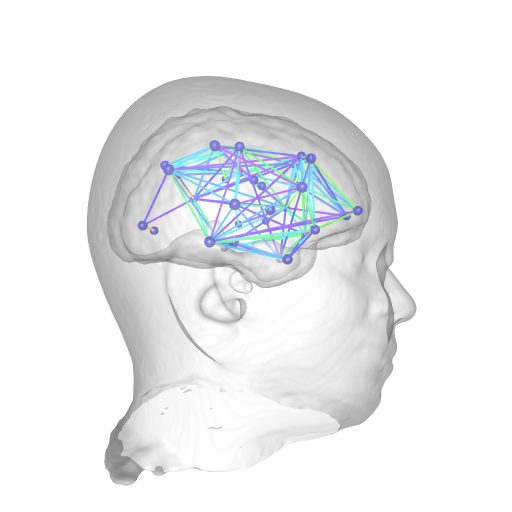
\includegraphics[width=55mm]{temp_female_network_R_70.png} \\
  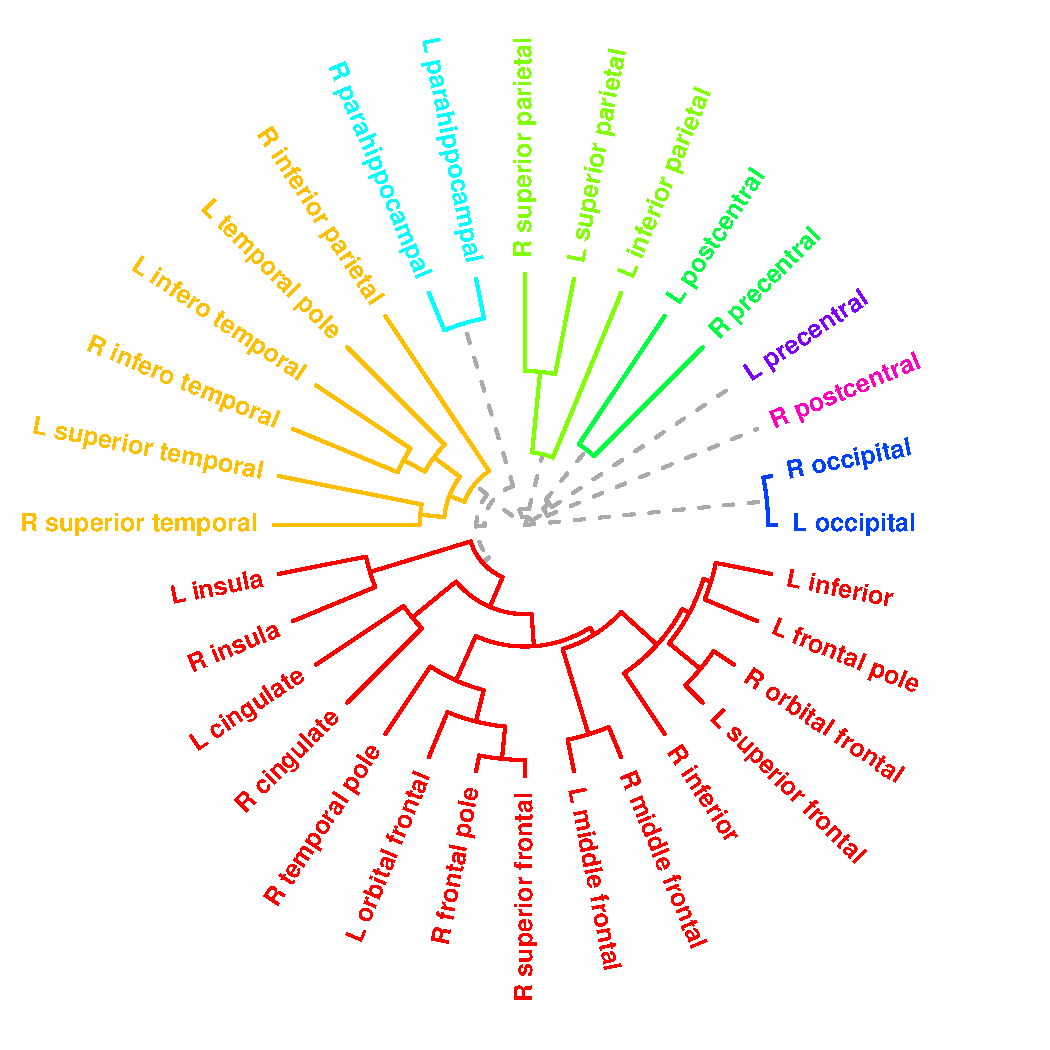
\includegraphics[width=55mm]{temp_female_community_X_20.pdf} &
  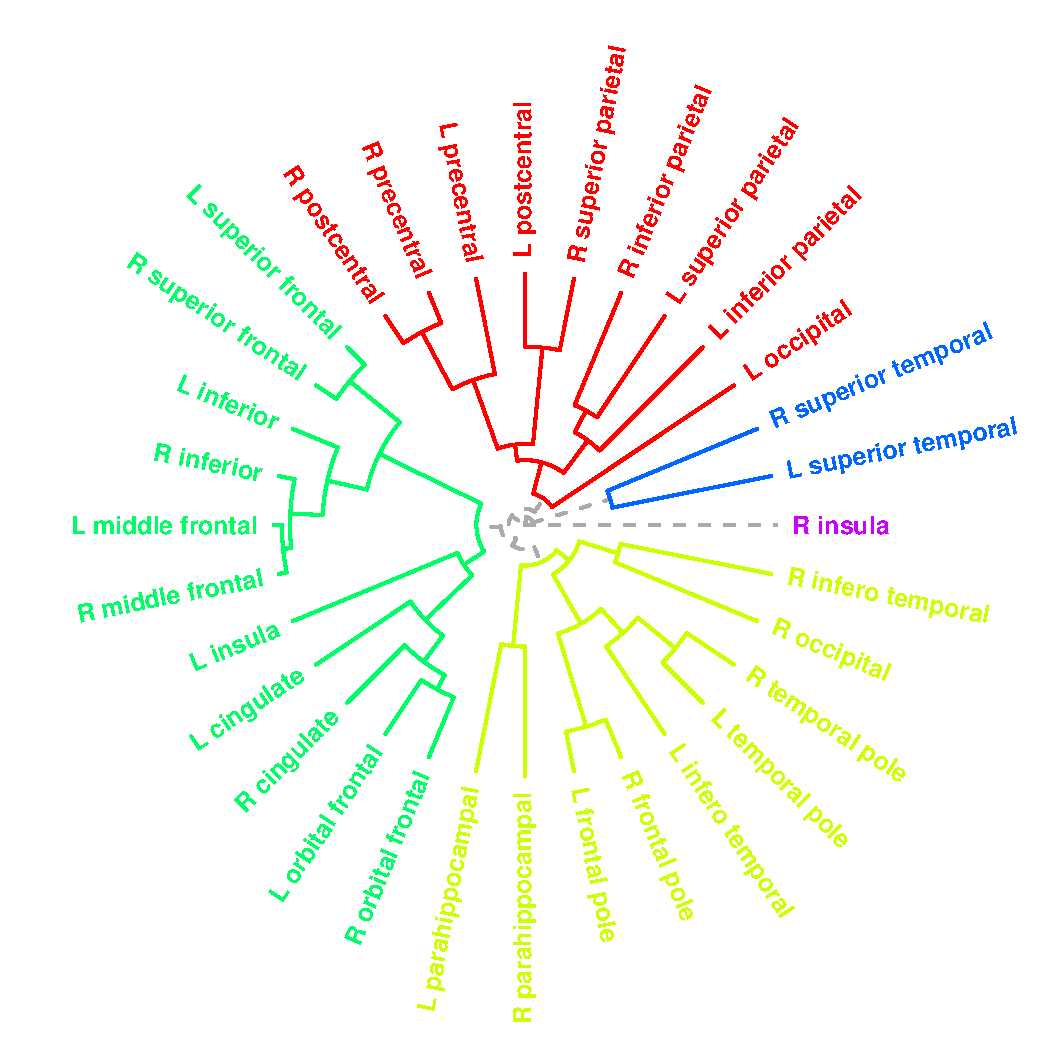
\includegraphics[width=55mm]{temp_female_community_X_40.pdf} &
  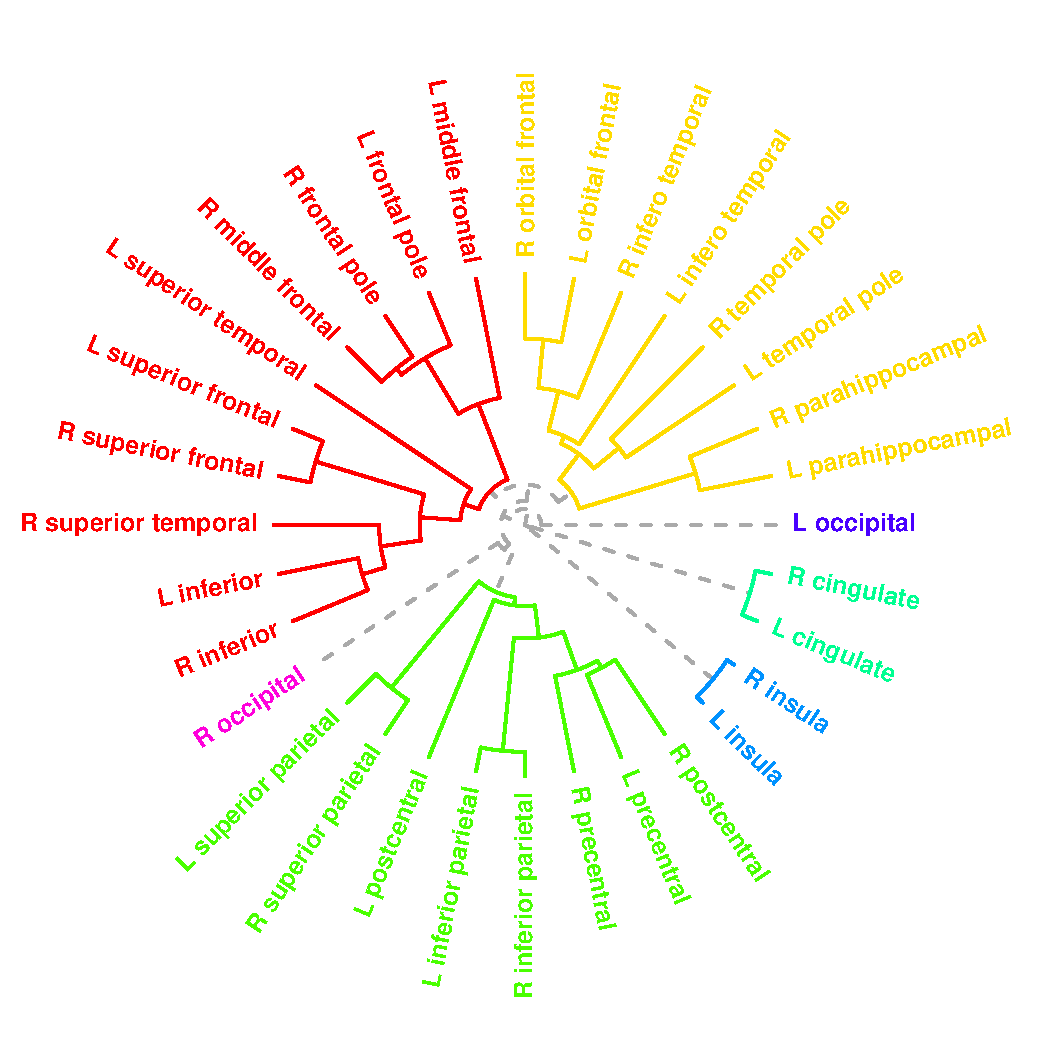
\includegraphics[width=55mm]{temp_female_community_X_70.pdf} \\
  20 years & 40 years & 70 years 
  \end{tabular}
  \caption{Visual illustration of the female thickness networks for ages 20, 40, 
  and 70 years.  Community relationships between regions are depicted both in 
  brain space (top row) and as a radial phylogenetic tree where colors denote 
  neighborhoods (bottom row).
  }
  \label{fig:femaleVisualNetworks}
\end{figure*}

\begin{figure*}[htb]
  \centering
  \begin{tabular}{ccc}
  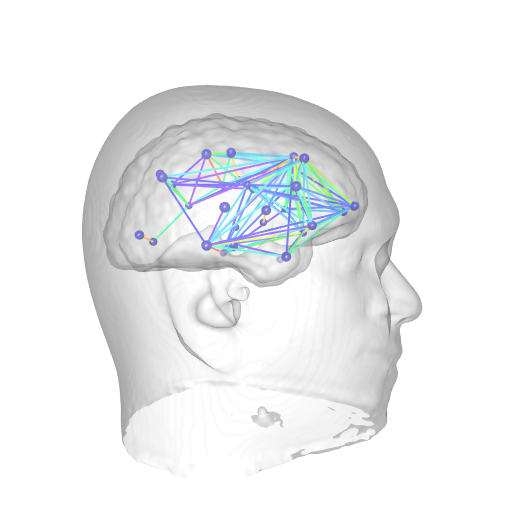
\includegraphics[width=55mm]{temp_male_network_R_20.png} &
  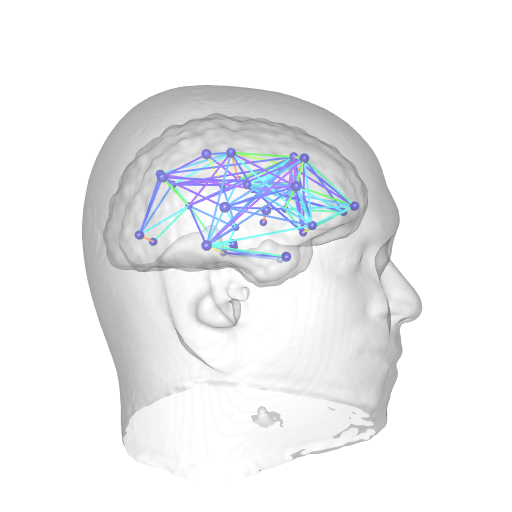
\includegraphics[width=55mm]{temp_male_network_R_40.png} &
  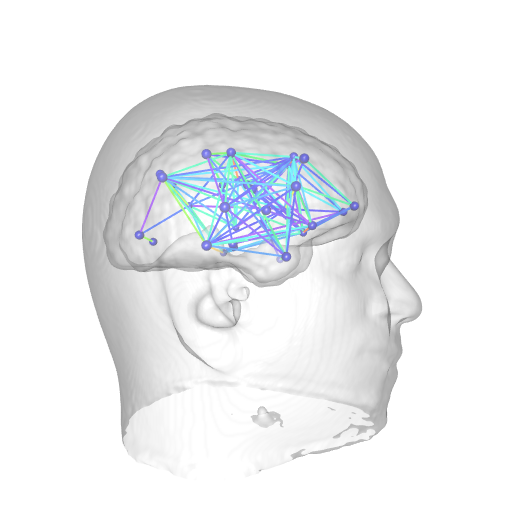
\includegraphics[width=55mm]{temp_male_network_R_70.png} \\
  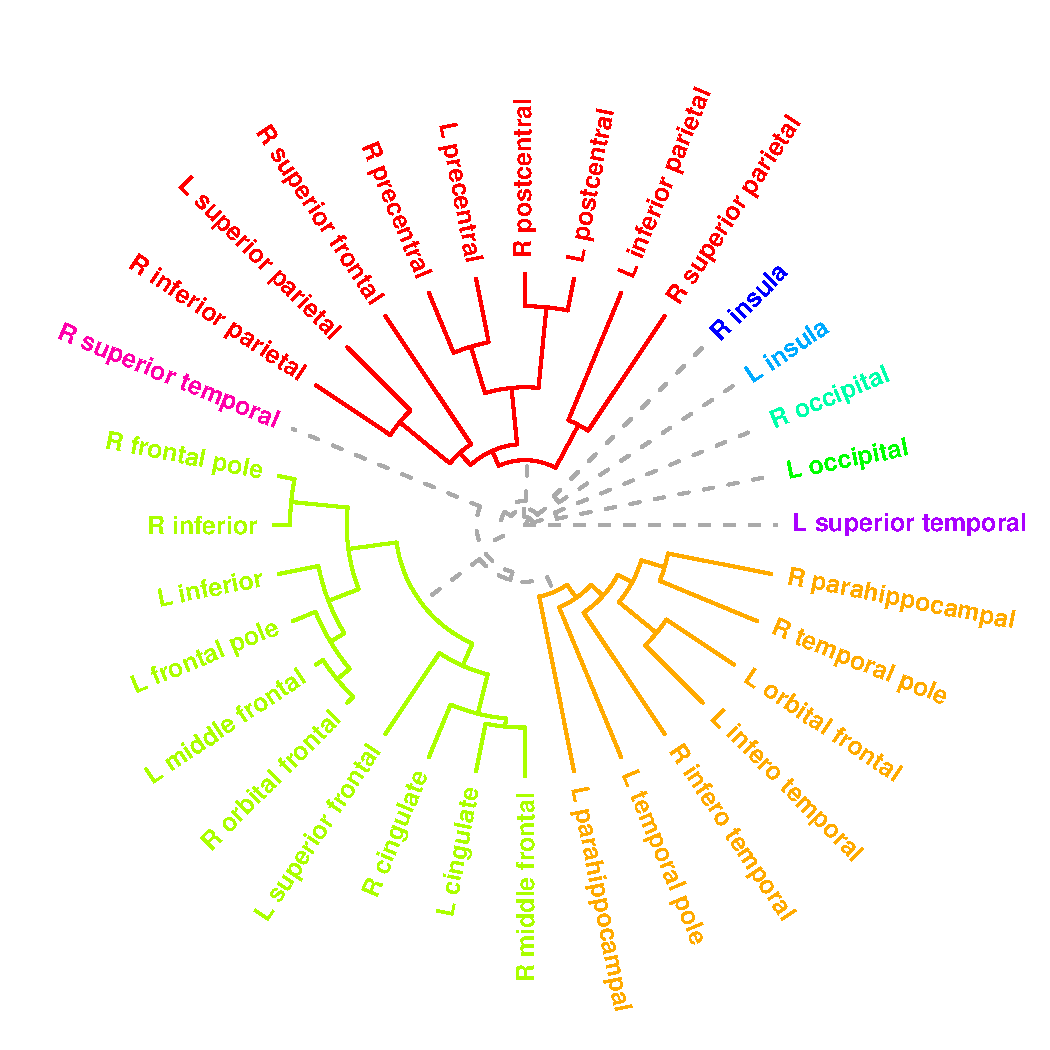
\includegraphics[width=55mm]{temp_male_community_X_20.pdf} &
  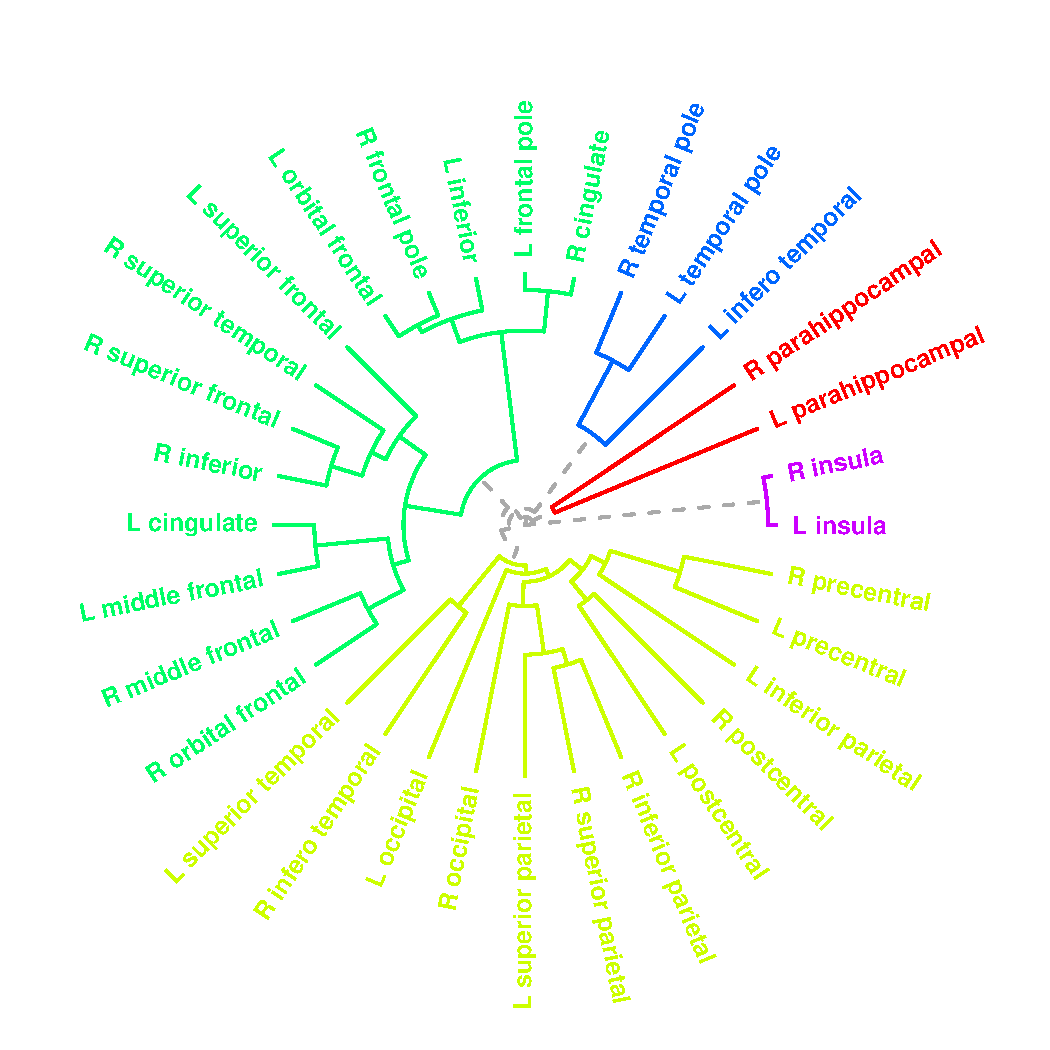
\includegraphics[width=55mm]{temp_male_community_X_40.pdf} &
  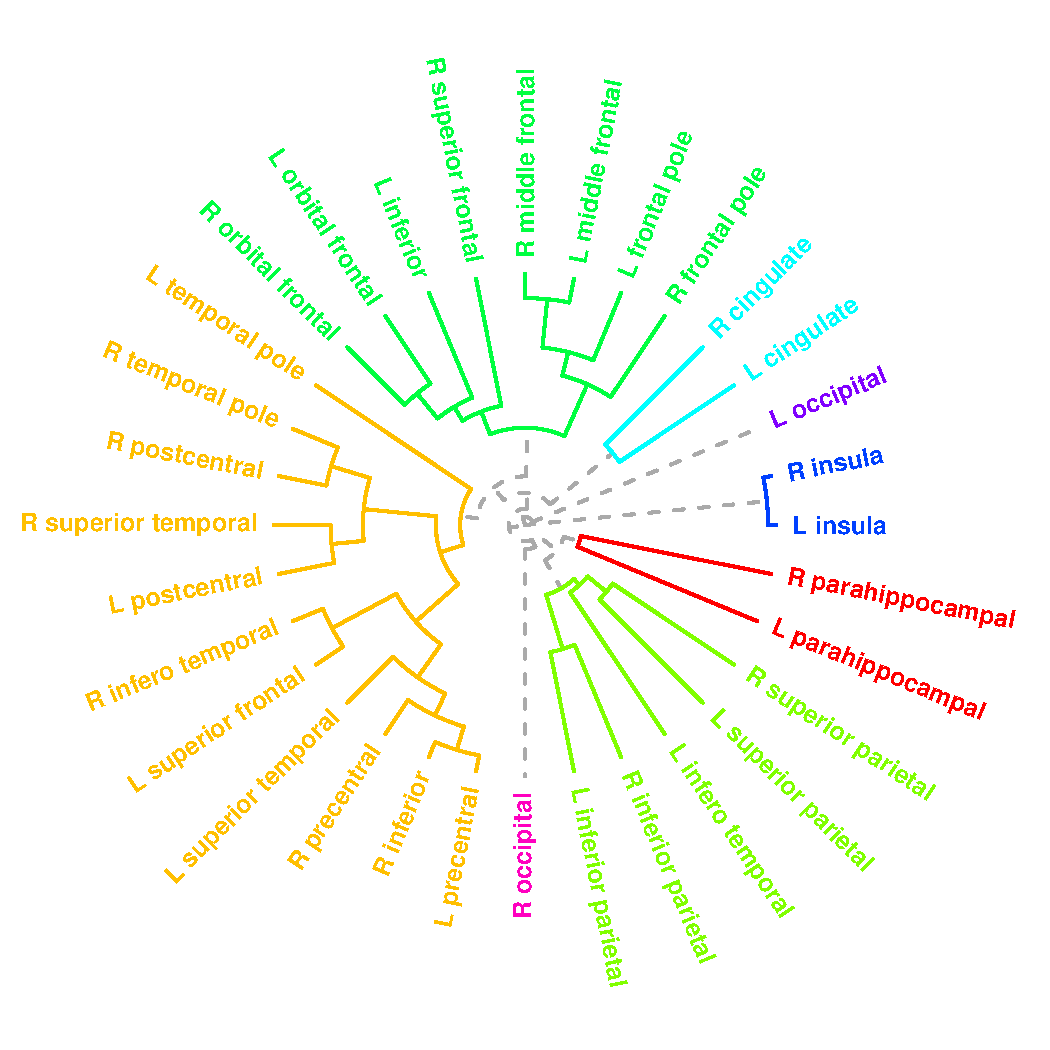
\includegraphics[width=55mm]{temp_male_community_X_70.pdf} \\
  20 years & 40 years & 70 years 
  \end{tabular}
  \caption{Visual illustration of the male thickness networks for ages 20, 40, 
  and 70 years.  Community relationships between regions are depicted both in 
  brain space (top row) and as a radial phylogenetic tree where colors denote 
  neighborhoods (bottom row).
  }
  \label{fig:maleVisualNetworks}
\end{figure*}



\begin{table}[htb]
\centering
\begin{tabular}{c l c c}
\toprule
Age & \multicolumn{1}{c}{Significant Regions} & Transitivity Diff. & $p$-value\\
\midrule
\rowcolor{gray!40}
10 & L superior frontal & 0.41 & 0.016 \\
\rowcolor{gray!40}
{} & R superior parietal & 0.40 & 0.048 \\
\rowcolor{gray!20}
15 & R superior frontal & 0.33 & 0.012 \\
\rowcolor{gray!20}
{} & L inferior & 0.33 & 0.027 \\
\rowcolor{gray!40}
20 & R insula & 1.0 & 0.0 \\
\rowcolor{gray!40}
{} & R superior frontal & 0.31 & 0.023 \\
\rowcolor{gray!20}
25 & R parahippocampal & 0.33 & 0.015 \\
\rowcolor{gray!40}
30 & L superior temporal & 1.0 & 0.0 \\
\rowcolor{gray!40}
{} & L inferior & 0.42 & 0.042 \\
\rowcolor{gray!40}
{} & L orbital frontal & 0.5 & 0.005 \\
\rowcolor{gray!40}
{} & L superior parietal & 0.6 & 0.002 \\
\rowcolor{gray!20}
35 & L superior temporal & 0.67 & 0.033 \\
\rowcolor{gray!20}
{} & R superior temporal & 0.81 & 0.012 \\
\rowcolor{gray!40}
40 & R inferior parietal & 0.68 & 0.001 \\
\rowcolor{gray!20}
45 & L parahippocompal & 1.0 & 0.0 \\
\rowcolor{gray!20}
{} & R superior frontal & 0.33 & 0.024 \\
\rowcolor{gray!20}
{} & R inferior & 0.42 & 0.016 \\
\rowcolor{gray!40}
50 & R parahippocampal & 0.57 & 0.03 \\
\rowcolor{gray!40}
{} & R superior temporal & 0.34 & 0.015 \\
\rowcolor{gray!20}
55 & L occipital & 0.56 & 0.018 \\
\rowcolor{gray!20}
{} & R occipital & 0.87 & 0.004 \\
\rowcolor{gray!40}
60 & R occipital & 0.72 & 0.0 \\
\rowcolor{gray!40}
{} & R orbital frontal & 0.44 & 0.024 \\
\rowcolor{gray!20}
65 & \multicolumn{1}{c}{---} & --- & --- \\
\rowcolor{gray!40}
70 & L parahippocampal & 0.83 & 0.042 \\
\rowcolor{gray!20}
75 & R parahippocampal & 0.83 & 0.018 \\
\rowcolor{gray!20}
{} & L frontal pole & 0.40 & 0.021 \\
\rowcolor{gray!20}
{} & L inferior parietal & 0.33 & 0.033 \\
\rowcolor{gray!40}
80 & L middle frontal & 0.39 & 0.022 \\
\rowcolor{gray!40}
{} & R inferior & 0.53 & 0.003 \\
\rowcolor{gray!40}
{} & R inferior parietal & 0.34 & 0.005 \\
\rowcolor{gray!40}
{} & R postcentral & 0.30 & 0.016 \\
\rowcolor{gray!20}
85 & R inferior parietal & 0.26 & 0.023 \\
\rowcolor{gray!40}
90 & \multicolumn{1}{c}{---} & --- & --- \\
\bottomrule
\end{tabular}
\caption{Regional gender differences in transitivity with age.  Statistical 
significance was determined using permutation testing ($n = 1000$).
}
\label{table:genderDifference}
\end{table}

\subsection{Quality Assessment Measures}
Considering the multiple components of the thickness protocol, there are 
several points at which a single subject processing failure can occur.  Initial mis-registration of the template can produce erroneous brain extraction results
which severely affects the remainder of the processing workflow.  Similarly,
incorrect segmentation results will negatively impact the cortical thickness measurements.
However, determining which individual subjects did not process correctly is a time-consuming task.  Although much of our quality assessment involved inspection of each
individual subject overlaid with the various processed images, an additional tool (which
we dub the {\em brain constellation map}) proved to be very useful as it provided a quick
assessment of results over the entire cohort and allowed for immediate identification
of problematic cases.%
\footnote{
  The script to create the brain constellation map is  {\tt makeThicknessStarsPlot.R}.
}  
A star plot of the thickness residuals 
($T(REGION_i) \sim AGE  + VOLUME+ SITE$) for each subject.
is in Figure \ref{fig:stars}. Subjects have been organized by 
increasing age and unique colors are assigned to each 
data set (IXI = red, Kirby = green, NKI = blue, Oasis = orange)
which permits visualization of age
distribution with data set.  Additionally, for each subject we
test for non-normality using the Shapiro-Francia normality test which
provides an additional measurement for quality assessment.

%  Nick:  We'll do all this later.
%\textcolor{red}{FIXME---should add an ``index'' to the constellation
%  map ... can be done with some parameter choice.  can be done later.
%do we want to show the old constellation map (pre 4-tissue)? or save
%as supplementary material ... }


 
\begin{figure*}
  \centering
  \begin{tabular}{c}
  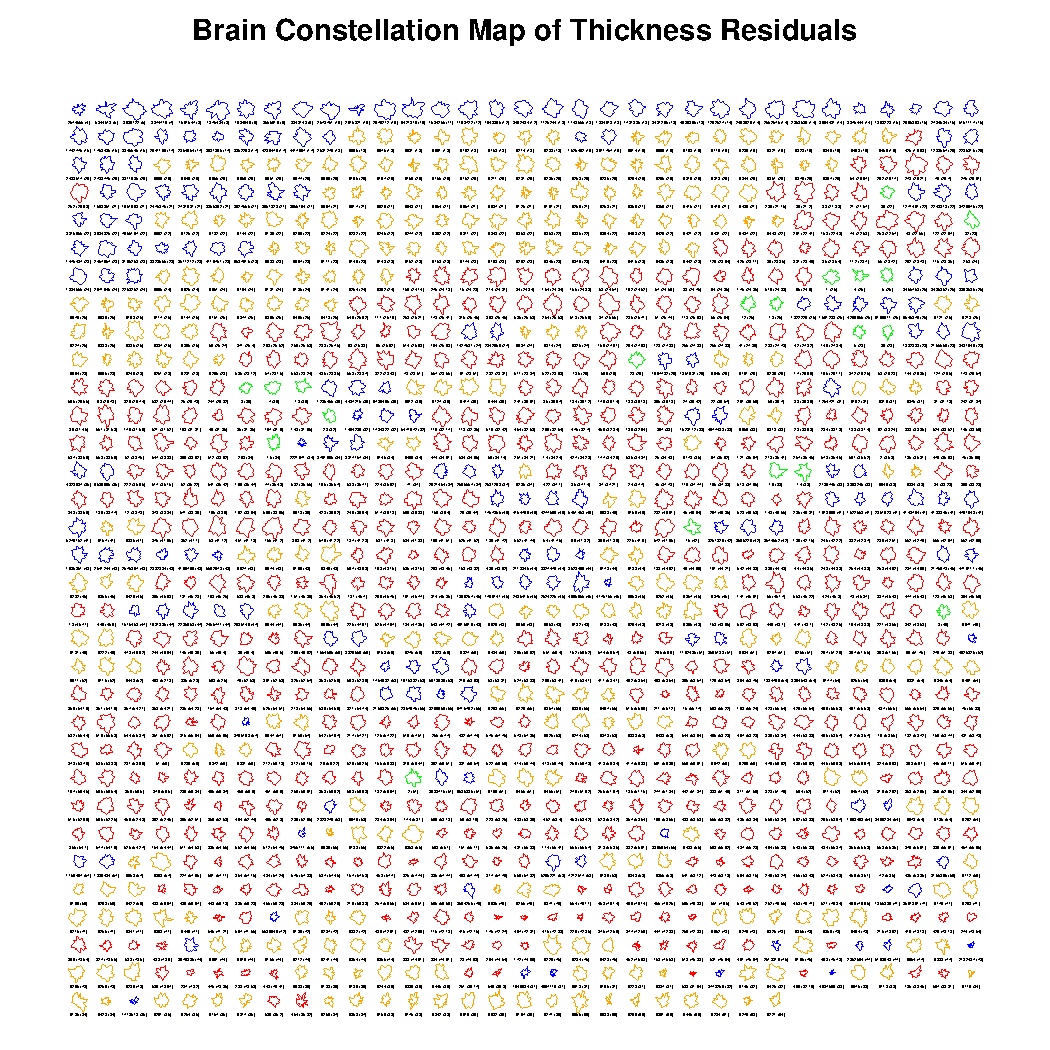
\includegraphics[width=180mm]{thicknessStarsIndividualsNew.pdf} 
  \end{tabular}
  \caption{Brain constellation map of the entire study cohort ordered left to right by age.  Thickness residuals for each of the 32 regions are rendered using star plots with color indicating the specific data set (IXI = red, Kirby = green, NKI = blue, Oasis = orange).  For quickly determining obvious processing failures, the figure can be magnified.  Below each subject is the ID, age, and a possible `*' denoting a significant result ($< 0.05$) of the Shapiro-Francia normality test \citep{royston1993} indicating non-normality. 
  }
  \label{fig:stars}
\end{figure*}






